
\subsubsection{Forward pass algorithm in \acrshort{rnn}}

The operation of the forward pass in an \acrshort{rnn} is similar to a normal layer. A basic recurrent layer usually has only one layer with the activation function such as $tanh$. The vector $h_{t}$ is a vector calculated by this activation function but that not only receives as parameter $x$, but also receives the previous hidden state $h_{t-1}$. In the same way, the vector $h_{t+1}$ will have information of both $h_{t}$ and $x_{t+1}$. As you can see, the hidden state of each layer is passed from layer to layer. Graphically:


\begin{figure}[H]
    \centering
    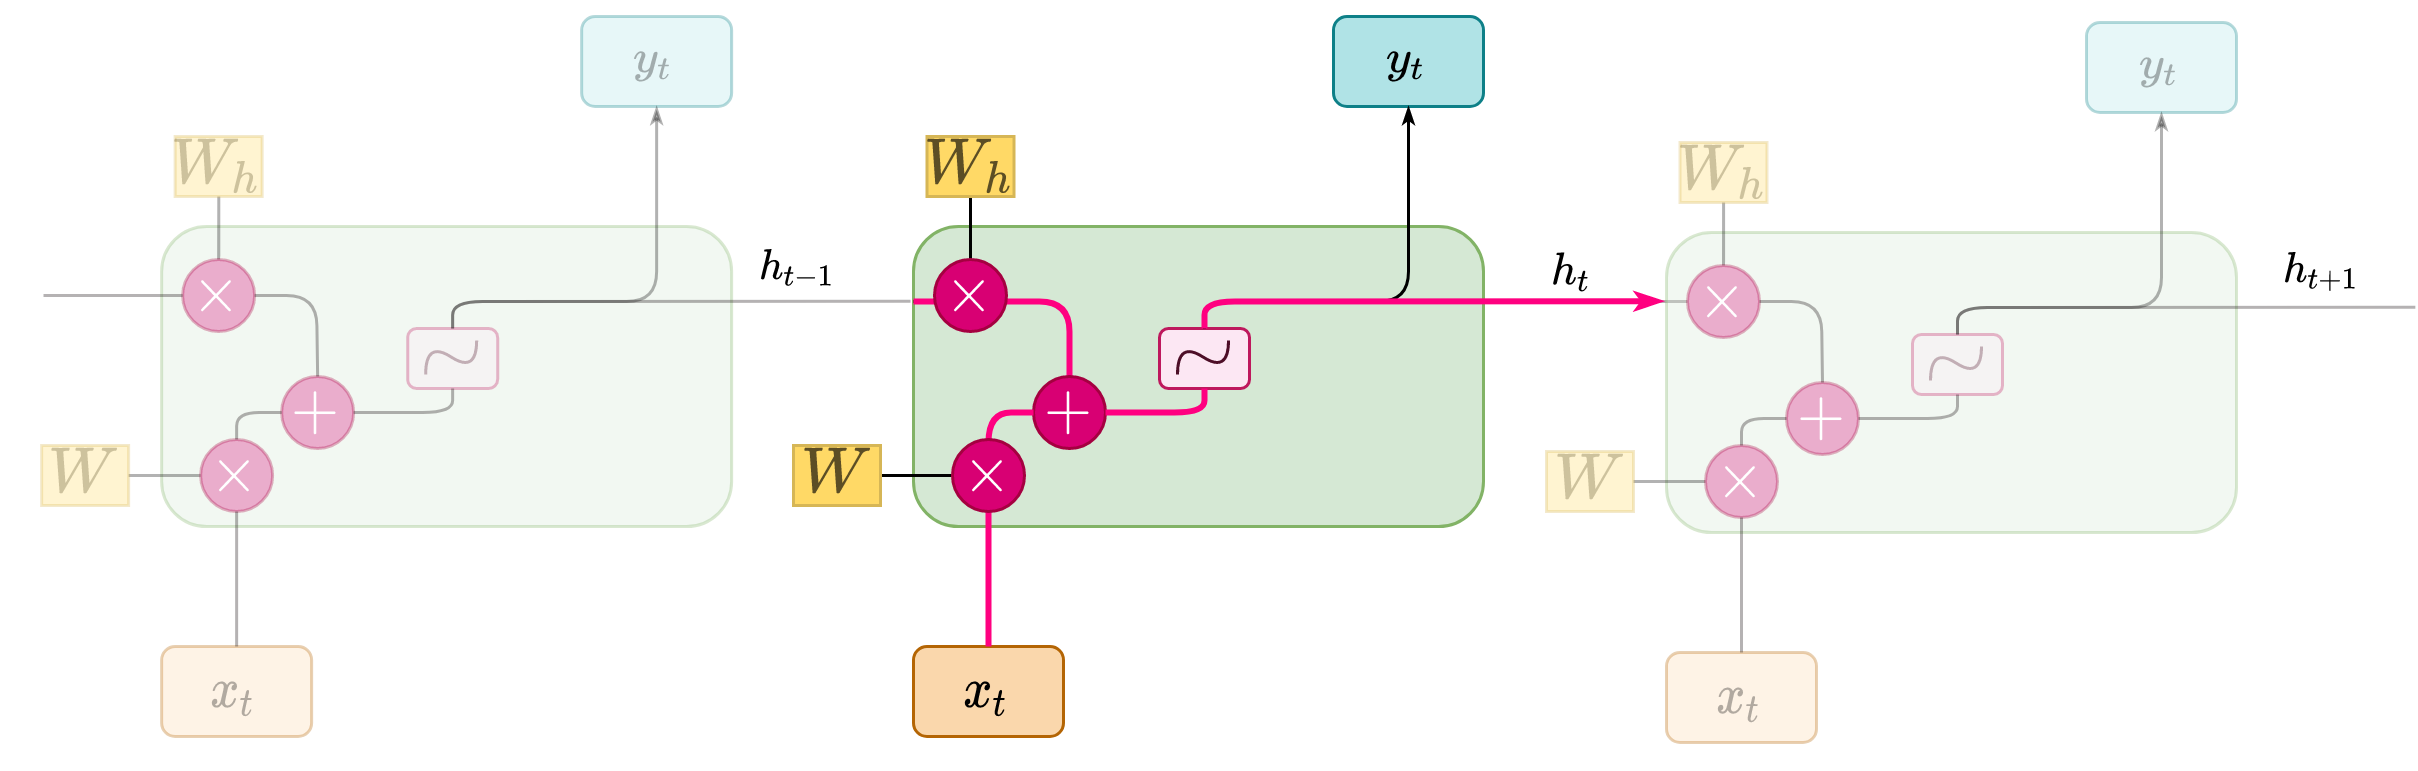
\includegraphics[width=14cm]{images/state-of-art/rnn/standard-rnn.png}
    \caption{Functioning of an \acrshort{rnn}.}
\end{figure}

 For each iteration, the presence of information from previous $h$ is reduced, causing the gradient to fade, a concept that will be explained later. This information flow can be better seen with the following diagram:


\begin{figure}[H]
    \centering
    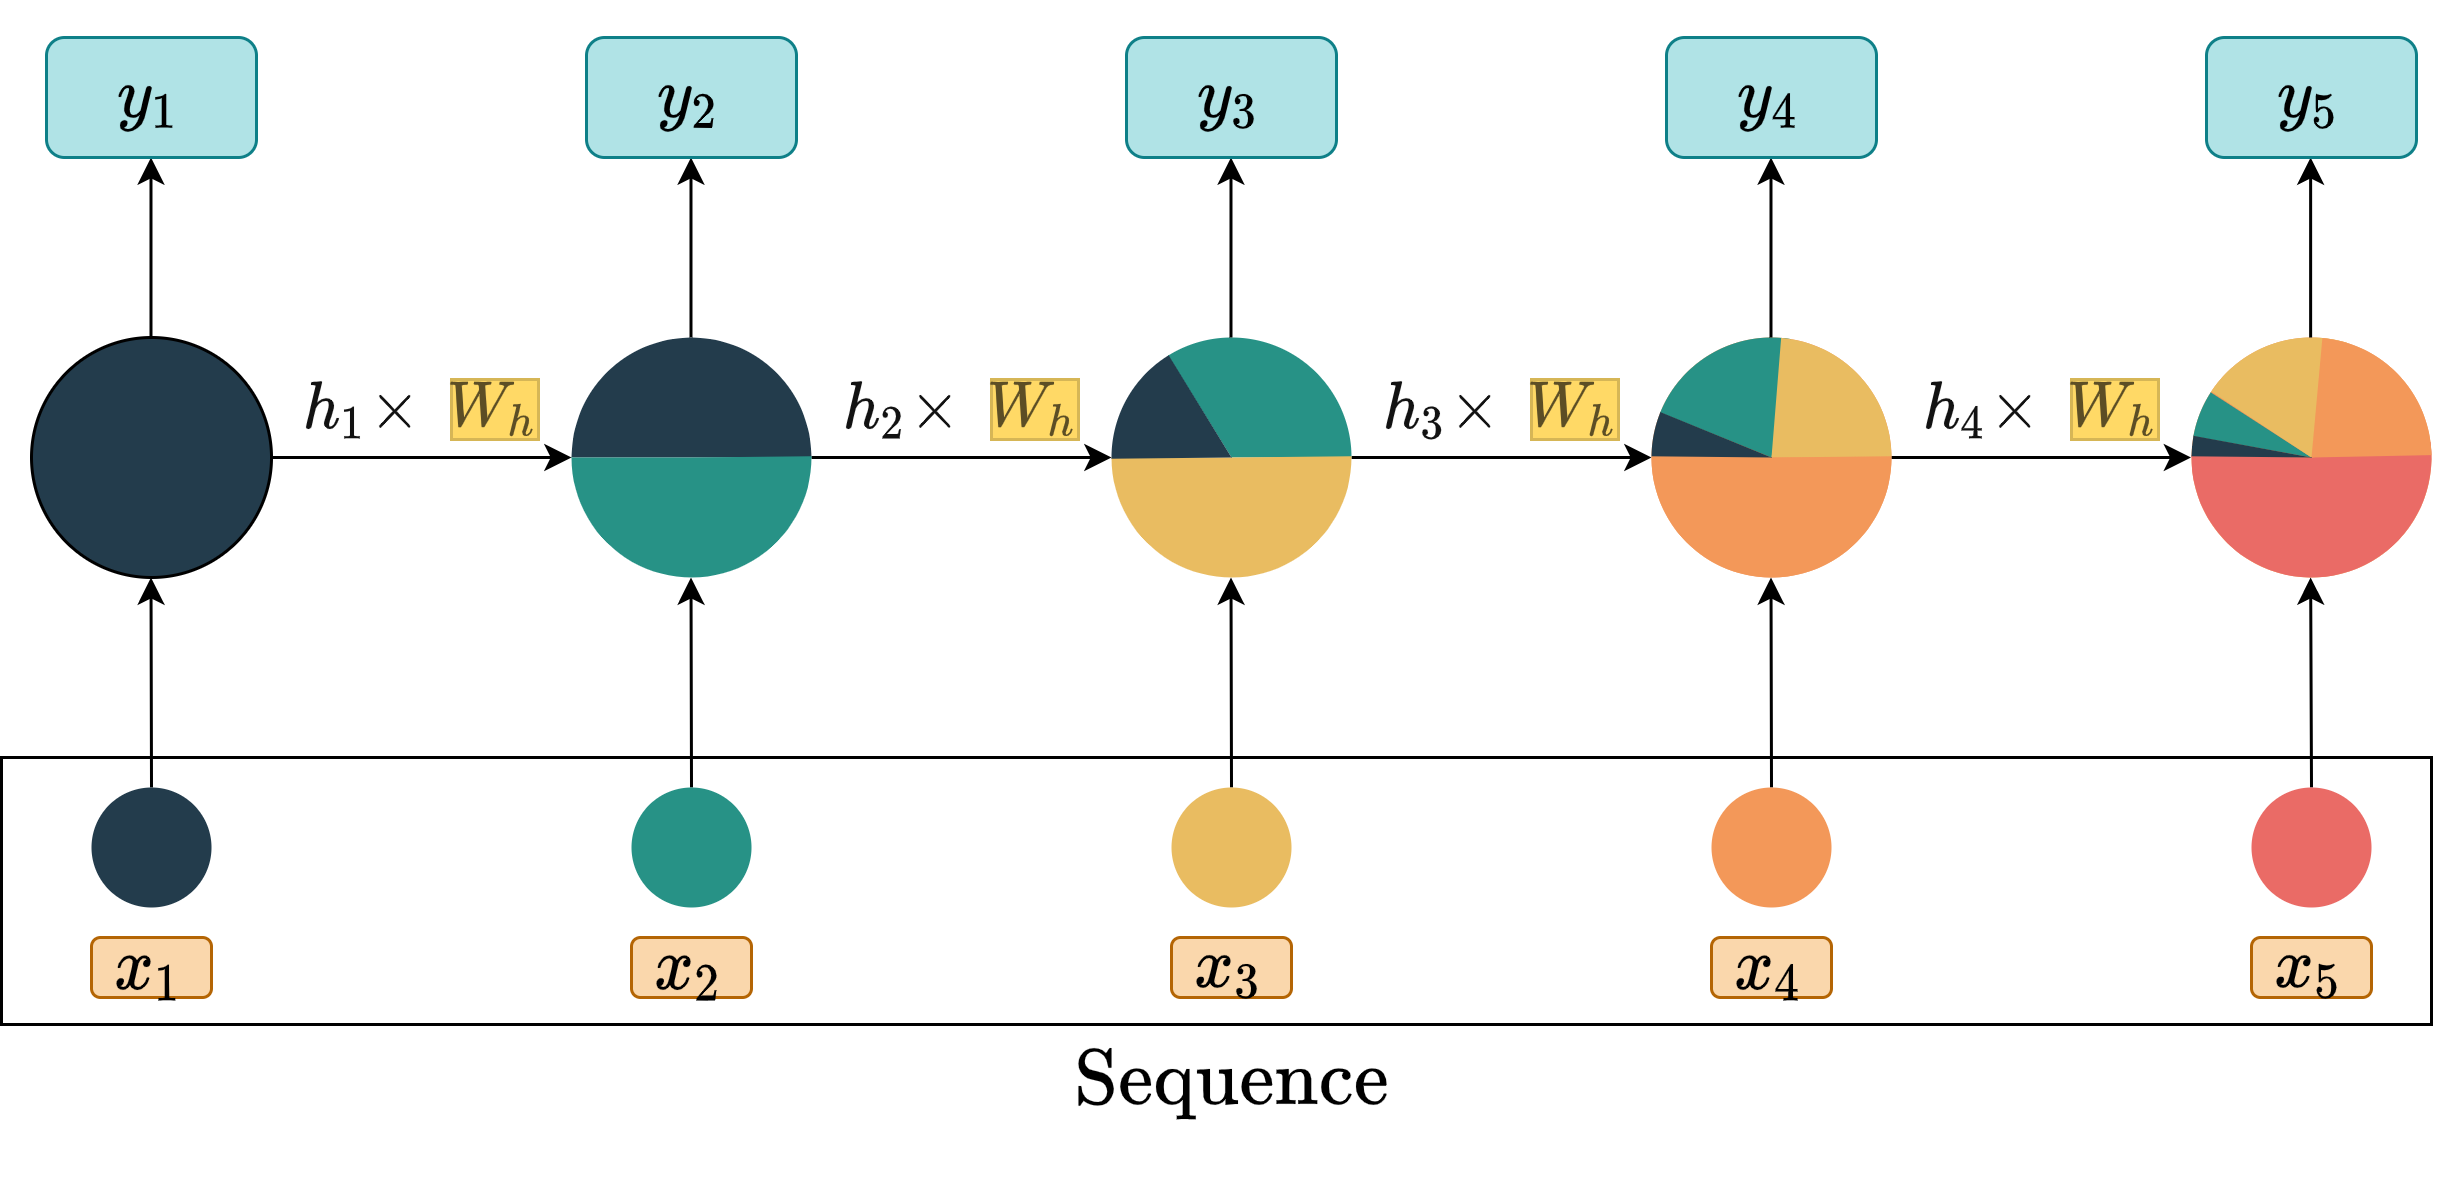
\includegraphics[width=11cm]{images/state-of-art/rnn/simple-rnn.png}
    \caption{Structure of a recurring layer}
    \label{fig:simple_rnn}
\end{figure}

The recurrent layers, as with the basic layers of a network, will have an associated matrix of weights (although they do not have biases $b$). This matrix will be represented with $W_h$ leaving $W$ for basic layer weight matrices. There can be multiple recurrent layers each one with an independent $W_h$ matrix, that is why the $RL_i$ index is used as explained in figure \ref{fig:rnn-compact}.
\newline


The calculation of $y$ is similar to the calculation in a normal neural network. Starting from the equation explained in equation \ref{eqn:feedforward}:
\begin{equation}
    y = a(W^{L_l} \cdot (a(W^{L_{l-1}} \cdot ... \cdot (a(W^{L_1} \cdot x')^{L_1})) \text{ } ... \text{ } ^{L_{l-1}}))^{L_l}
\end{equation}

Simplifying this calculation to a single layer:
\begin{equation}
    \begin{split}
        z &= W^{L_l} \cdot y^{L_i} \\
        y &= a(z)
    \end{split}
\end{equation}

If it is a recurrent layer, a new summation has to be added to the operation, but we want it to continue to have the same properties of the activation function, so in reality, what is going to be modified is the calculation of $z$:
\begin{equation}
    \begin{split}
        z &= W^{L_l} \cdot y^{L_i} + W_h \cdot h \\
        y &= a(z)
    \end{split}
\end{equation}


For example, if you have a recurrent network made up of five layers, where the first and third layers are recurrent, the calculation of final $y$ is as follows:

\begin{equation}
    y = a(W^{L_5} \cdot a(W^{L_4} \cdot a(W^{L_3} \cdot a(W^{L_2} \cdot a(W^{L_1} \cdot x' + W_h^{RL_1} \cdot h_1 ))^{L_2} + W_h^{RL_2} \cdot h_2)^{L_3})^{L_4})^{L_5}
\end{equation}


The calculation of $z$ will depend on whether the recurring layer is the first one:
\begin{equation}
    z^{L_1} = W^{L_1} \cdot x' + W_{h} \cdot h
\end{equation}

Otherwise, if the recurring layer is not the first one:
\begin{equation}
    z^{L_i} = W^{L_i} \cdot y^{L_{i-1}} + W_{h} \cdot h
\end{equation}

